\chapter{i-vectorの抽出精度向上のための発話区間結合手法}
\label{chapter:prob_method}
\ref{section:pre_cos}節より、短い発話データからは話者の特徴を十分に抽出できないことが確認された。インデクシングを行う上で、アンカーの発話区間検出と音声認識ではi-vectorが用いられているため、i-vectorの抽出精度を向上させることでさらなるアンカーの発話区間の検出精度と音声認識精度の向上が見込めると考えた。そのため、ニュース番組特有の特徴である「同じ話者が連続で発話すること」「話者によって発話環境が異なること」の2点に着目して同じ話者の発話区間であると考えられる発話区間を結合することで擬似的に長い発話を作成し、i-vectorの抽出精度を向上させることを目指した。本稿では、2通りの方法で前後の同一話者と考えられる発話区間を結合する。1つ目は発話間の時間情報を考慮した発話区間の結合手法である。2つめは、話者の発話環境を考慮した発話区間の結合手法である。図\ref{fig:indexing2}は、本稿の提案手法を組み込んだインデクシング手法の流れである。

\begin{figure}[H]
  \begin{center}
    \includegraphics[scale=0.3]{./figure/indexing2.eps}
  \end{center}
  \caption{提案手法を組み込んだインデクシング手法 \label{fig:indexing2}}
\end{figure}

\section{発話間の時間情報を考慮した発話区間の結合手法}
本手法では、発話区間と発話区間の間(非発話区間)が短い場合、発話区間を結合する。これは図\ref{fig:same_sp}で示されるように、同一話者が連続で発話する場合は間をおかずに次の発話を行うことが非常に多く、非発話区間が非常に短いためである。つまり、非発話区間が非常に短いとき、高い確率で同一話者の発話が行われると考えられる。しかし、話者が切り替わった場合でも対話中やインタビューイの存在により非発話区間が非常に短い場合がある。この場合、同一話者が連続で発話しているか話者が切り替わったかの判別は非発話区間の時間情報のみでは不可能である。そこで、図\ref{fig:iv_same_short}と図\ref{fig:iv_other_short}より、発話が非常に短い場合でも若干のコサイン類似度の差があることに着目した。これらより、非発話区間が非常に短く、発話から抽出されたi-vectorのコサイン類似度が一定値以上のとき、同一話者の発話と判別し発話区間を結合する。

\section{発話環境を考慮した発話区間の結合手法}
本手法では、発話環境の変化を音源識別によって検出し、同一話者の可能性が高い前後の発話区間を結合する。ニュース番組にはスタジオにいるアンカーや天気アナウンサーのほか、台風の状況を中継する中継アナウンサー、騒音の中でインタビューを受けるインタビューイなどが存在する。そこで、アンカーから中継アナウンサー、インタビューイからアンカーなど話者が切り替わった場合発話環境が変化することに着目した。しかし、音源識別では、発話の背景雑音がどの種類であるかを特定することが非常に難しい。そこで、非発話区間の音源識別結果を用いることで、発話環境の変化を検出する。発話環境の変化の検出方法を以下の図に示す。\par

\begin{figure}[H]
  \begin{center}
    \includegraphics{./figure/same_sp.eps}
  \end{center}
  \caption{同一話者間の非発話区間の時間情報 \label{fig:flow_prob2}}
\end{figure}

例の図\ref{fig:flow_prob2}では、最初の話者の非発話区間が「無音区間」であることから、雑音が少ない環境で発話していることがわかる。ここで、次の話者が発話を始めたとき、発話環境が「雑音区間」に変化している。つまり、雑音の多い屋外などで発話をしているインタビューイや中継アナウンサーに話者が切り替わったと考えられる。ここで、前の非発話区間と現在の非発話区間の音源識別結果を参照し、同一の結果であった場合発話区間を結合、異なった場合、話者の切り替わりと識別する。
